\documentclass[letterpaper, 12pt]{article}
\linespread{1.5} 
\author{Nicola Corbellini\thanks{\footnotesize Department of Economics, Pennsylvania State University. Email: \href{mailto:nzc5436@psu.edu}{nzc5436@psu.edu}. 
\\I thank the Enterprise Analysis Unit of the Development Economics Global Indicators Group of the World Bank for the data, and Josh Wimpey for useful clarifications regarding the World Bank Enterprise Survey microdata. All errors are my own.}}
\date{\today}
\title{Measuring Informal GDP Using Survey Data}

\usepackage{mathpazo}
% \usepackage{fourier}
\usepackage[margin=1in]{geometry}
\usepackage{amsmath}
\usepackage{xcolor}
\usepackage{bbm}
\usepackage{amssymb}
\usepackage[nottoc]{tocbibind}
\usepackage{amstext} 
\usepackage{eurosym}
\usepackage{float} 
\DeclareRobustCommand{\officialeuro}{%
  \ifmmode\expandafter\text\fi
  {\fontencoding{U}\fontfamily{eurosym}\selectfont e}}
  \usepackage{graphicx}
\usepackage{caption}
\usepackage{subcaption}
\usepackage{footnote}
\makesavenoteenv{table}
\makesavenoteenv{tabular}
\renewcommand{\baselinestretch}{1.25}
% \usepackage[round]{natbib}
\usepackage[authordate]{biblatex-chicago}
\addbibresource{mybibfile.bib}
\usepackage[hidelinks]{hyperref}
\usepackage{setspace} \setstretch{1.5}
% \usepackage{fancyhdr}
% \pagestyle{fancy}
% \fancyhf{} 
% \renewcommand{\headrulewidth}{0pt}
% \fancyfoot[RO]{\thepage}
% \fancypagestyle{plain}{%
%   \fancyhf{}
%   \fancyfoot[RO]{\thepage}
%   \renewcommand{\headrulewidth}{0pt}
% }
\usepackage{multirow}
\addtolength{\skip\footins}{2pc plus 5pt}
% \renewcommand{\thesection}{\Roman{section}} 
% \renewcommand{\thesubsection}{\thesection.\Alph{subsection}}


\begin{document}

\maketitle

\begin{abstract}
    \begin{singlespace}
    This paper estimates the share of informal GDP in 26 developing countries over a period that spans up to 2004–2023. The focus is on the concept of legal informality, defined as the activities of enterprises that are not formally registered. I propose a simple framework that formally characterizes informal GDP. I use data from various sources, including the World Bank Enterprise Survey and the International Labour Organization (ILO), to match the conditions derived from the framework. The resulting informality series conform to patterns documented in previous research, such as a negative correlation with GDP per capita and mild anticyclical behavior. Because I adopt a narrower definition of informality, the estimated levels tend to be lower than those reported in previous cross-country studies.
    \end{singlespace}
\end{abstract}

% \vspace{1cm}

\section{Introduction}
A large share of economic activity in developing countries occurs within the informal sector. However, consistently measuring informality across countries presents several challenges. First, surveys often adopt varying definitions of informality. For example, some focus on different units, such as firms or employees, or emphasize different dimensions, such as the activities of unregistered firms rather than unreported activities of otherwise formal firms. Second, existing measures of informality rely on two main approaches, each with its own strengths and limitations. Direct methods, such as employment and enterprise surveys, ensure representativeness within a country and do not rely on strong assumptions, but are available for only a limited number of countries and years and are less suitable for cross-country comparisons. In contrast, indirect methods facilitate comparability across countries but rely on statistical or economic models characterized by strong assumptions about the relationship between informality and other economic variables. 
\\This paper adopts a combination of direct and indirect methods to estimate the share of informal GDP in 26 developing countries over a period that spans up to 2004–2023, depending on the country. I focus on the concept of \textit{legal informality}, defined as the economic activities of enterprises that are not formally registered. Compared to broader definitions, this approach excludes informal activities conducted by otherwise formal enterprises. From a methodological perspective, I introduce a simple framework that formally characterizes the concept of informal GDP. A key contribution of this paper is the use of statistics from the World Bank Enterprise Survey (WBES) to match some of the conditions derived from the proposed framework. Specifically, I use firm-level data to compute average sales and value added per worker in both the formal and informal sectors. This information is then combined with data on formal and informal employment from the International Labour Organization (ILO), along with other macroeconomic variables. The constructed series are designed so that fluctuations in informal GDP are primarily driven by changes in informal employment, as reported by the ILO. For each country, I derive two series of informal GDP: one based on average sales per worker, the other on average value added per worker. Since the former likely underestimates informal GDP, while the latter likely overestimates it, these two series can be interpreted as lower and upper bounds, respectively.
\\The estimated measures of informal GDP are negatively correlated with GDP per capita. However, some low-income countries exhibit relatively low levels of informality. This finding is not in contradiction with previous research, which has highlighted that factors beyond the stage of economic development, such as institutions or tax enforcement, also influence informality. Regarding the evolution of informality over time, two patterns stand out. First, some countries maintain a stable level of informality throughout the period considered, while others experience a gradual decline. Second, the series exhibit a mild anticyclical behavior, aligning with previous studies documenting increases in informality during recessions. Finally, the estimated levels of informal GDP are somewhat lower than those reported in previous cross-country studies. This discrepancy is likely due to the narrower concept of informality adopted here, which excludes, for example, unreported activities conducted by formal enterprises.
\\The remainder of the paper is organized as follows. Section \ref{sec_def} provides an overview of the definitions and measurement approaches related to informality. 
Section \ref{sec_model} introduces the framework used to estimate informal GDP. Section \ref{sec_data} describes the data used. Section \ref{sec_results} discusses the main features of the estimated informality series. Section \ref{sec_concl} concludes.
\\
\\
\noindent
\textbf{Related literature.} This paper contributes to the literature estimating the size of the informal economy. Much of the existing research focuses on specific dimensions of informality or on individual countries. For example, \textcolor{blue}{\textcite{orsietal2014}} develop a \textit{dynamic general equilibrium} (DGE) model with an informal sector to estimate the size and evolution of the underground economy in Italy, while \textcolor{blue}{\textcite{dinolaetal2021}} analyze the size and effects of tax evasion in the US.
\\Some studies, however, provide broader cross-country estimates of informality. \textcolor{blue}{\textcite{schneideretal2010}} adopt a \textit{multiple indicators multiple causes} (MIMIC) approach to measure informality across 162 countries from 1999 to 2007. The main idea behind the MIMIC method is to retrieve an unobserved variable (share of informal GDP) using structural equations and the sample covariances between observed variables (e.g., self-employment and other macroeconomic variables).  \textcolor{blue}{\textcite{elginoztunali2012}} develop a DGE model in which a representative household allocates labor between the formal and informal sectors.  The model is then calibrated using national account statistics to estimate the size of the shadow economy in 161 countries from 1950 to 2009.\footnote{For both \textcolor{blue}{\textcite{schneideretal2010}} and \textcolor{blue}{\textcite{elginoztunali2012}}, updated series up to 2018 are available in \textcolor{blue}{\textcite{elginetal2021}}.} While this paper derives measures of informality for a narrower set of countries and years, it offers three key advantages over previous works. First, the base-year \textit{levels} are derived from firm-level data rather than alternative methods such as the currency demand approach. Second, \textit{changes} over time are mainly driven by changes in labor force survey statistics, rather than shifts in some of the national account statistics used to calibrate the model. Third, I introduce a quantitative estimate of a narrower concept of informality, namely legal informality, which is often conflated with other measures in earlier studies. Another relevant work is \textcolor{blue}{\textcite{pappadarogoff2025}}, who propose a measure of the informal economy based on the discrepancy between national account data and VAT tax records. The authors derive measures of informality for countries across the European Union during the period 1999–2020. Their approach, while more transparent and less dependent on model assumptions, focuses on a smaller group of developed economies and emphasizes a particular dimension of informality, namely tax evasion. 
\\This paper also relates to previous work describing the main characteristics of informality. For example, \textcolor{blue}{\textcite{laportashleifer2014}} document its prevalence in low- and middle-income countries and its negative correlation with GDP per capita. Along with other country-specific studies such as \textcolor{blue}{\textcite{ulyssea2018}}, they also highlight
the smaller size and lower productivity of informal businesses. This aligns with the paper's finding that the share of employment outside the formal sector exceeds the share of GDP produced outside the formal sector. Finally, the anticyclical behavior of informality observed in the estimated series has been previously documented, for example, by \textcolor{blue}{\textcite{leyvaurrutia2020}} and \textcolor{blue}{\textcite{pappadarogoff2025}}. 


\section{Informality: Definitions and Measurements}\label{sec_def}
\textbf{Definitions.}
I follow the categorization proposed by the \textcolor{blue}{\textcite{worldbank2020}}, which distinguishes between three degrees of informality: (i) \textit{legal informality}, referring to the business registration status, (ii) \textit{fiscal informality}, concerning compliance with taxes and regulations, and (iii) \textit{labor informality}, reflecting the type of contracts and benefits available to employees. The measure of informality used in this paper focuses on legal informality. Specifically, I employ data from the ILO and the WBES to collect employment and other balance sheet information of unregistered businesses operating in the informal sector. According to the \textcolor{blue}{\textcite{ilo}}, an informal sector business or enterprise  
(i) is unregistered and unincorporated, (i.e., it is not constituted as a legal entity separate from its owners) and (ii) it sells at least some of the goods or services it produces. This definition is consistent with the one adopted by the World Bank in its Informal Sector Enterprise Survey (ISES). In fact, the ISES focuses on businesses that lack a business license, do not exist on a business registry, and/or are not registered with the relevant tax authority (\textcolor{blue}{\textcite{agaetal2022}}).
\\
\\\textbf{Measurements.}
There exist two main approaches to measuring informality: \textit{direct methods} and \textit{indirect methods}.
Direct methods are collected from labor force surveys, household surveys, enterprise surveys, or a combination thereof. These approaches typically capture several dimensions of informality, such as business and employment informality.  
Their main advantage is that they require minimal assumptions. However, their infrequent implementation makes it difficult to obtain estimates that cover a broad range of countries and years. Moreover, cross-country comparisons are not always possible given the differences in the implementation of the surveys and/or the definitions of informality across countries. 
\\Indirect methods, by contrast, involve statistical or economic models that link measures of informality with other observed economic variables. These methods can produce time series that are more comparable across countries and years, but they rely heavily on specific assumptions and are therefore subject to model misspecification.  
\\As detailed in the next section, I combine direct methods, such as statistics derived from ILO and World Bank data, with indirect  methods, including the specification of an aggregate production function, to estimate informal GDP shares for a group of developing countries.


\section{Informality Accounting}\label{sec_model}
I consider a model economy in which aggregate output $Y$ is the sum of output produced in the formal sector, $Y_F$, and output produced outside the formal sector, $Y_O$. In both sectors, there is a representative firm that transforms production inputs into output. Specifically, the formal sector's representative firm employs capital and labor to produce output, while the informal sector's representative firm employs labor only:
\begin{align}
    Y_F&=\theta_F K_F^{\alpha}N_F^{\gamma_F}\nonumber\\
    Y_O&=\theta_O N_O^{\gamma_O}\nonumber
\end{align}
Where $K_F$ denotes formal sector's capital, $N_F$ and $N_O$ denote total employment in the formal and informal sector, $\alpha$ is the capital share in the formal sector, $\gamma_F$ and $\gamma_O$ are the labor share in the formal and informal sectors, and $\theta_F$ and $\theta_O$ denote TFP terms in the two sectors.
\\The objective is to derive the share of informal GDP $S_O$:
\begin{equation}
    S_O=\frac{Y_O}{Y}=\frac{\theta_O N_O^{\gamma_O}}{\theta_F K_F^{\alpha}N_F^{\gamma_F}+\theta_O N_O^{\gamma_O}}\label{info_share}
\end{equation}
\noindent
Note that $\theta_O$ and $\theta_F$ are the only unknowns in equation (\ref{info_share}). I use employment series from ILO and capital series from the Penn World Table (PWT), while the production factor shares are estimated using data from the WBES. From this survey, I also compute country-level averages of sales per worker in the formal and informal sectors. Let the sales per worker averages be $\mu_F$ and $\mu_O$. Therefore, for the years in which the WBES is conducted, I use the following two equations to derive $\theta_F$ and $\theta_O$:
\begin{align}
    \frac{Y_F}{N_F}&=\theta_F K_F^{\alpha}N_F^{\gamma_F-1}=\mu_F\label{vapw_form}\\
    \nonumber\\
    \frac{Y_O}{N_O}&=\theta_O N_O^{\gamma_O-1} = \mu_O\label{vapw_info}
\end{align}
This procedure allows me to derive estimates of informal GDP only for the years in which the WBES is conducted. I make the following assumptions to extend these measures backward and forward over time: (i) the estimated factor shares $\alpha$, $\gamma_F$, and $\gamma_O$ are constant over time, (ii) the growth rates of TFP in the two sectors $\delta\theta_{F,t} = \frac{\theta_{F,t}-\theta_{F,t-1}}{\theta_{F,t-1}}$ and $\delta\theta_O=\frac{\theta_{O,t}-\theta_{O,t-1}}{\theta_{O,t-1}}$ are such that $\delta\theta_F=\delta\theta_O$, and (iii) $\theta_{F,t}$ and $\theta_{O,t}$  satisfy the following equation for each year $t$ in which employment data from the ILO are available:
\begin{equation}
    \delta(\theta_{F,t} K_{F,t}^{\alpha}N_{F,t}^{\gamma_F}+\theta_{O,t} N_{O,t}^{\gamma_O}) = \delta(GDP_t)\label{eq_gdpgr}
\end{equation}
Where $\delta(GDP_t)$ denotes the GDP growth rate $\frac{GDP_t-GDP_{t-1}}{GDP_{t-1}}$. $GDP_t$ growth rates are taken from PWT and, for the most recent years, the World Bank. Equation (\ref{eq_gdpgr}) states that the growth rate of the TFP measures $\theta_{F,t}$ and $\theta_{O,t}$ is such that the model-implied growth rate of output equals the measured growth rate of GDP.
\\I then repeat the same steps using averages of value added per worker, in place of sales per worker, in the formal and informal sectors in equations (\ref{vapw_form}) and (\ref{vapw_info}). In Section \ref{sec_results}, I present two distinct time series of informality for each country, one based on sales per worker and the other on value added per worker. While value added is a more appropriate measure than gross sales for assessing the relative contribution of the two sectors, firm-level data on intermediate purchases are sometimes missing. This limitation reduces both the size and representativeness of the samples in the value added-based series.

\section{Data}\label{sec_data}
\textbf{WBES.} I use data from the WBES to estimate the production function's factor shares and to compute average sales and value added per worker in the formal and informal sectors.\footnote{The raw data used for this project are publicly available at \\ \href{https://www.enterprisesurveys.org/en/enterprisesurveys}{https://www.enterprisesurveys.org/en/enterprisesurveys}} Specifically, I combine data from the standard WBES, which samples registered firms with at least five employees, and the ISES, which targets informal businesses.\footnote{The Appendix provides more details concerning WBES data.} Both surveys focus exclusively on the non-agricultural sector. In addition, firm-level information is available on sector (manufacturing or services), number of employees, and annual sales. Sample weights are available for all observations in the formal sample, while they are available only for informal surveys conducted after 2016. Consequently, I assign equal weights to all observations within a country from informal surveys prior to 2016. Table \ref{tab_sales} lists the number of firm-level observations, and the (weighted) average number of employees and yearly sales for each country, separately for the formal and informal sectors.


\begin{table}[ht!]
    \caption{Summary Statistics (Sales).}
    \label{tab_sales}
\scriptsize
    \centering
    \begin{tabular}{ll|ccc|ccc}
     &  & & \textbf{Formal Sector} & & & \textbf{Informal Sector} & \\
     & &  & \textbf{Average} & \textbf{Average} &  & \textbf{Average} & \textbf{Average} \\
     \textbf{Country}& \textbf{Year} & \textbf{Obs.} & \textbf{Employment} & \textbf{Sales} & \textbf{Obs.} & \textbf{Employment} & \textbf{Sales} \\
        & & &  & \textbf{(Th. 2017 USD)} &  &  & \textbf{(Th. 2017 USD)} \\
\hline
\hline
% Afghanistan & 2008 & 456 & 24.61 & 2935.5 & 329 & 9.6 & 191.2 \\
Burkina Faso & 2009 & 372 & 28.66 & 2247.4 & 102 & 3.6 & 20 \\
Cameroon & 2009 & 347 & 52.42 & 5509.7 & 121 & 3.04 & 14.9 \\
% Cape Verde & 2009 & 147 & 21.37 & 28617.7 & 74 & 2.23 & 97 \\
Cote d'Ivoire & 2009 & 508 & 16.11 & 1458.1 & 97 & 2.78 & 7.8 \\
Madagascar & 2009 & 355 & 59.56 & 1476.5 & 123 & 2.07 & 4.5 \\
Mauritius & 2009 & 383 & 44.93 & 5891.5 & 122 & 1.53 & 18.7 \\
Nepal & 2009 & 363 & 13.93 & 323.7 & 120 & 4.09 & 16.8 \\
Niger & 2009 & 137 & 16.93 & 3115.9 & 108 & 5.25 & 10.3 \\
Angola & 2010 & 323 & 34.06 & 308203.3 & 78 & 9.23 & 625 \\
Argentina & 2010 & 971 & 72.58 & 10866.4 & 308 & 1.59 & 6 \\
Botswana & 2010 & 232 & 61.61 & 8748.3 & 95 & 2.69 & 13.1 \\
Guatemala & 2010 & 435 & 96.1 & 5211.2 & 278 & 1.78 & 5.9 \\
Mali & 2010 & 248 & 19.92 & 3350.6 & 85 & 4.53 & 16.3 \\
Rwanda & 2011 & 190 & 36.14 & 1514.5 & 190 & 2.38 & 4.6 \\
% Congo, The Democratic Republic of & 2013 & 481 & 22.07 & 10559.9 & 444 & 3.14 & 12.1 \\
Egypt & 2013 & 2443 & 39.18 & 1140.6 & 74 & 3.96 & 14 \\
% Kenya & 2013 & 660 & 57.27 & 8365.3 & 478 & 1.57 & 5.6 \\
Myanmar & 2014 & 540 & 31.6 & 303.7 & 276 & 5.41 & 39.5 \\
Zimbabwe & 2016 & 600 & 31.88 & 1325.7 & 499 & 1.96 & 8.7 \\
Lao, People's Democratic Republic & 2018 & 300 & 19.11 & 695.5 & 351 & 2 & 7.9 \\
% Mozambique & 2018 & 601 & 40.45 & 1191.5 & 474 & 1.6 & 1.1 \\
Zambia & 2019 & 563 & 67.01 & 2112.7 & 659 & 1.87 & 1.6 \\
Bangladesh & 2022 & 966 & 114.84 & 1556.6 & 2851 & 6.99 & 14.9 \\
Ghana & 2022 & 664 & 27.83 & 904.9 & 2652 & 1.91 & 4.2 \\
India & 2022 & 9319 & 20.56 & 756.3 & 8471 & 1.64 & 5 \\
% Iraq & 2022 & 780 & 21.63 & 432.4 & 1572 & 2.29 & 13.7 \\
Peru & 2022 & 939 & 38.82 & 3368.5 & 1294 & 1.39 & 3.9 \\
Sudan & 2022 & 248 & 28.53 & 644764.4 & 1345 & 1.82 & 8.3 \\
Cambodia & 2023 & 519 & 94.89 & 1073.3 & 1277 & 1.57 & 3.6 \\
% Central African Republic & 2023 & 139 & 20.76 & 38.2 & 1308 & 1.47 & 1.4 \\
Indonesia & 2023 & 2237 & 23.14 & 1035.1 & 4896 & 1.52 & 5.7 \\
Tanzania, United Republic of & 2023 & 513 & 22.5 & 176 & 1377 & 1.54 & 1.4 \\\hline
\hline
\end{tabular}
    \caption*{Source: Own calculation based on WBES.}
\end{table}

\noindent
Based on the available balance sheet data from the surveys, I compute value added differently across the two sectors. In the formal sector, value added is calculated by subtracting the value of intermediate goods purchases from annual sales. In the informal sector, where data on intermediate purchases are rarely available, I approximate value added by subtracting total electricity costs from annual sales. Table \ref{tab_va} shows the number of available observations along with (weighted) averages of the number of employees and value added for both sectors in each country. Note that the employment figures differ from those displayed in Table \ref{tab_sales} because some observations are dropped when computing value added.

\begin{table}[ht!]
    \caption{Summary Statistics (Value Added).}
    \label{tab_va}
\scriptsize
    \centering
    \begin{tabular}{ll|ccc|ccc}
     &  & & \textbf{Formal Sector} & & & \textbf{Informal Sector} & \\
     & &  & \textbf{Average} & \textbf{Average} &  & \textbf{Average} & \textbf{Average} \\
     \textbf{Country}& \textbf{Year} & \textbf{Obs.} & \textbf{Employment} & \textbf{Value Added} & \textbf{Obs.} & \textbf{Employment} & \textbf{Value Added} \\
        & & &  & \textbf{(Th. 2017 USD)} &  &  & \textbf{(Th. 2017 USD)} \\
\hline
\hline
% Afghanistan & 2008 & 76 & 36.24 & 335.2 & 147 & 9.44 & 170.3 \\
Burkina Faso & 2009 & 52 & 38.24 & 1806.4 & 97 & 3.71 & 19.7 \\
Cameroon & 2009 & 90 & 91.94 & 10664.7 & 113 & 3 & 14.6 \\
% Cape Verde & 2009 & 63 & 19.94 & 510.8 & 64 & 2.28 & 99 \\
Cote d'Ivoire & 2009 & 158 & 25.63 & 2056.5 & 89 & 2.73 & 7.8 \\
Madagascar & 2009 & 149 & 107.9 & 535.6 & 120 & 2.08 & 4.4 \\
Mauritius & 2009 & 138 & 67.61 & 2174.6 & 120 & 1.54 & 15.8 \\
Nepal & 2009 & 240 & 13.71 & 68.2 & 120 & 4.09 & 16.5 \\
Niger & 2009 & 35 & 18.44 & 272.1 & 93 & 5.27 & 7.6 \\
Angola & 2010 & 129 & 44.62 & 171004.8 & 51 & 7.82 & 761 \\
Argentina & 2010 & 658 & 81.86 & 7975.9 & 246 & 1.51 & 5.7 \\
Botswana & 2010 & 71 & 50.9 & 1567.6 & 85 & 2.74 & 13.5 \\
Guatemala & 2010 & 241 & 77.57 & 2276.3 & 254 & 1.78 & 5.9 \\
Mali & 2010 & 40 & 49.97 & 399.1 & 65 & 4.77 & 13.9 \\
Rwanda & 2011 & 38 & 83.03 & 1440.1 & 151 & 2.47 & 5 \\
% Congo, The Democratic Republic of & 2013 & 201 & 42.37 & 33516.8 & 435 & 3.16 & 12 \\
Egypt & 2013 & 1632 & 48.54 & 818.8 & 74 & 3.96 & 14 \\
% Kenya & 2013 & 291 & 113.16 & 11970.9 & 386 & 1.58 & 5.5 \\
Myanmar & 2014 & 266 & 68.71 & 328.6 & 270 & 5.4 & 39.6 \\
Zimbabwe & 2016 & 280 & 42.26 & 1885.5 & 307 & 2.01 & 6.6 \\
Lao, People's Democratic Republic & 2018 & 121 & 30.2 & 253.1 & 283 & 1.79 & 8 \\
% Mozambique & 2018 & 252 & 66.38 & 1141.9 & 438 & 1.61 & 1 \\
Zambia & 2019 & 155 & 108.17 & 1256.9 & 162 & 1.83 & 2.3 \\
Bangladesh & 2022 & 506 & 167.26 & 681 & 1941 & 9.88 & 19 \\
Ghana & 2022 & 162 & 44.11 & 646.7 & 1237 & 2.25 & 4.1 \\
India & 2022 & 5209 & 29.11 & 652.6 & 3872 & 1.77 & 4.5 \\
% Iraq & 2022 & 254 & 14.77 & 611.6 & 664 & 2.37 & 12 \\
Peru & 2022 & 354 & 58.63 & 2188.6 & 415 & 1.52 & 4 \\
Sudan & 2022 & 18 & 52.42 & 2833.3 & 756 & 1.84 & 9.4 \\
Cambodia & 2023 & 260 & 346.14 & 2333 & 926 & 1.61 & 2.8 \\
% Central African Republic & 2023 & 21 & 21.59 & 48.1 & 920 & 1.46 & 1.4 \\
Indonesia & 2023 & 865 & 39.26 & 970.3 & 3377 & 1.53 & 5.5 \\
Tanzania, United Republic of & 2023 & 150 & 18.65 & 118.6 & 710 & 1.69 & 1.6 \\
\hline
\hline
\end{tabular}
    \caption*{Source: Own calculation based on WBES.}
\end{table}

\noindent
To estimate the formal sector's production function shares $\alpha$ and $\gamma_F$, I run the following country-specific regressions:
\begin{equation}\label{eq_prod_form}
    ln \ y_i = \beta_0 + \alpha \ ln \ k_i + \gamma_F \ln \ l_{F,i}+\rho_t+\rho_s+\varepsilon
\end{equation}
\noindent
Where $y_i$, $k_i$, and $l_{F,i}$ denote value added, capital, and number of employees of formal firm $i$, respectively, while $\rho_t$ and $\rho_s$ are year and sector fixed effects.\footnote{Year fixed effects are included in the regressions since the survey year does not always coincide with the year of operations.} Value added and capital are expressed in 2017 USD. 
\\For the informal sector, I run the following specification:
\begin{equation}\label{eq_prod_info}
    ln \ y_i = \beta_0 + \gamma_O \ln \ l_{O,i}+\rho_t+\rho_s+\varepsilon
\end{equation}
Where $l_{O,i}$ denotes the number of employees of informal firm $i$.
I can then obtain country-specific estimates of $\alpha$, $\gamma_{F}$, and $\gamma_{O}$ that are used in equations (\ref{vapw_form}) - (\ref{eq_gdpgr})

\vspace{3mm}
\noindent
\textbf{ILO.} I use data from the International ILO to obtain measures of formal and informal employment. For informal employment, I rely on the \textit{number of employees outside the formal sector} in non-agriculture for individuals aged 15 or more. This measure includes workers employed in at least one informal sector enterprise, defined as an unregistered and unincorporated enterprise (there is no legal entity separated from its owners) that sells at least some of the goods or services it produces. Note that this definition is consistent with the one used in the WBES. 
\\The ILO harmonizes informality series by processing  microdata files from national household survey using a consistent navigational path, ensuring that the resulting statistics are comparable across countries.
However, I implement some adjustments to the ILO time series to address a few gaps and inconsistencies. First, I discard series whose figures are markedly inconsistent with preceding or subsequent surveys. In nearly all such cases, the survey source differs from the others available for the same country (e.g., a household survey instead of labor force surveys). Second, informal employment data are typically available only for a subset of years. When this occurs, I linearly interpolate employment values for the missing years using data from the available years. The graphs presented in Section \ref{sec_results} clearly distinguish between years with observed employment data and those with interpolated values.
\\To compute formal sector employment, I subtract employment outside the formal sector from \textit{total employment} in non-agriculture sector for individuals aged 15 or more.\footnote{The raw total and informal employment data are available at \href{https://ilostat.ilo.org/data/}{https://ilostat.ilo.org/data/}.}  
\\
\\
\noindent
\textbf{PWT and World Bank.}
I use data from the PWT for the time series on capital and GDP.\footnote{PWT data are taken from \textcolor{blue}{\cite{feenstraetal2015}}, available for download at \href{www.ggdc.net/pwt}{www.ggdc.net/pwt}.} Since the most recent version of the PWT includes data up to 2019, I extend the series using data from the World Bank. Specifically, for the capital series, I update the PWT data by adding investment, measured as gross capital formation, and subtracting capital depreciation:
$$K_{t}=(1-\delta)K_{t-1}+I_t, \ \ \ \ \ for \ t\geq2020$$
Where $K_{t}$ denotes capital, $I_t$ denotes investment, while $\delta$ is the country-specific average depreciation rate between 2002 and 2019 taken from PWT.
\\However, capital and GDP series from PWT and the World Bank include the agricultural sector, which may lead to inconsistencies with the WBES data that focus exclusively on the non-agricultural sector. For this reason, I scale the GDP series by multiplying it by (1-$S_A$), where $S_A$ is the share of agricultural GDP from the WB, and I apply the same adjustment to the capital series. This approach assumes that the share of aggregate capital in the non-agricultural sector is equal to the non-agricultural share of GDP.

\section{Results}\label{sec_results}
Figures \ref{info_ser_1} to \ref{info_ser_4} display the informality series for 26 countries. The solid black lines represent the share of employees operating outside the formal sector, which is taken from ILO as the ratio between employment outside the formal sector and total employment in non-agriculture for individuals aged 15 or more. The dashed blue lines show the share of fiscal informality calculated using average sales per worker in the two sectors on the right-hand side of equations (\ref{vapw_form}) and (\ref{vapw_info}). The dotted red lines, instead, reflect calculations based on average value added per worker. Finally, diamonds indicate years for which informal employment data are available from ILO. Interpolated data are used when direct observations are unavailable. The following terminology is adopted throughout this section: the solid black lines are referred to as \textit{informal employment}, the dashed blue lines as \textit{sales-based informal GDP}, and the dotted red lines as \textit{VA-based informal GDP}.

% \newpage 
    \begin{figure}[ht!]
        \centering
        \caption{Measures of Informality for Selected Countries}\label{info_ser_1}
        \begin{subfigure}[b]{0.49\textwidth}
            \centering
            \caption{}
            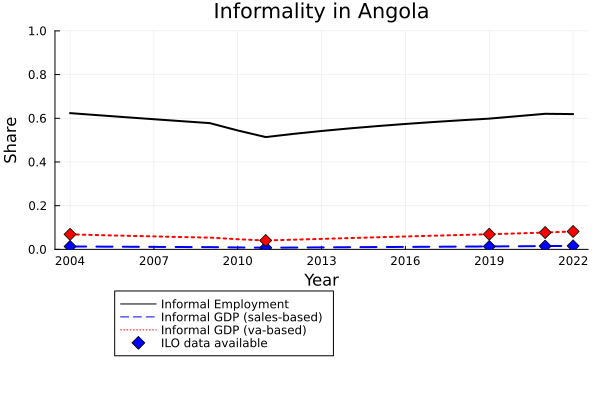
\includegraphics[width=\textwidth]{Angola.png}
        \end{subfigure}
        \hfill
        \begin{subfigure}[b]{0.49\textwidth}
            \centering
            \caption{}
            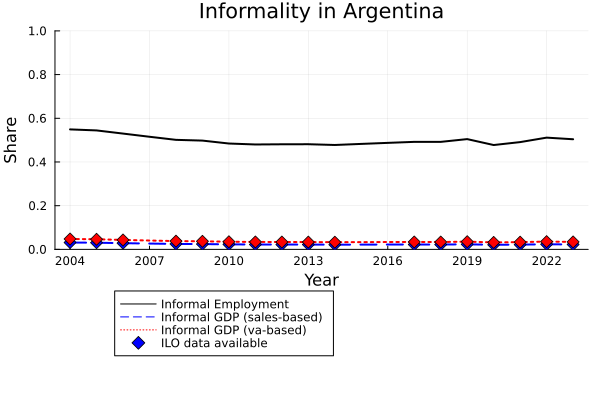
\includegraphics[width=\textwidth]{Argentina.png}
        \end{subfigure}
                \begin{subfigure}[b]{0.49\textwidth}
            \centering
            \caption{}
            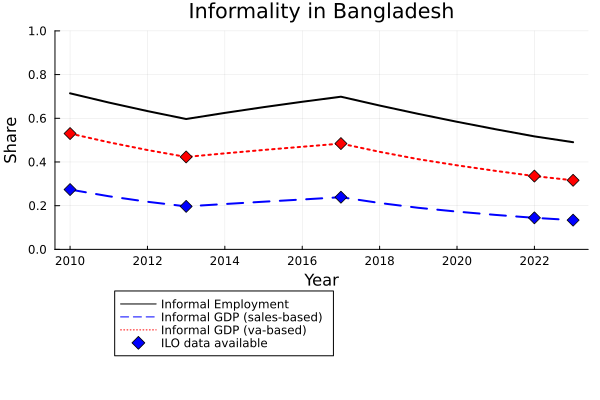
\includegraphics[width=\textwidth]{Bangladesh.png}
        \end{subfigure}
        \hfill
        \begin{subfigure}[b]{0.49\textwidth}
            \centering
            \caption{}
            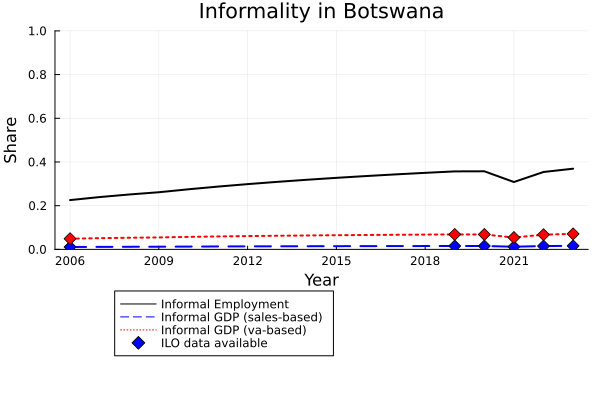
\includegraphics[width=\textwidth]{Botswana.png}
        \end{subfigure}
                \begin{subfigure}[b]{0.49\textwidth}
            \centering
            \caption{}
            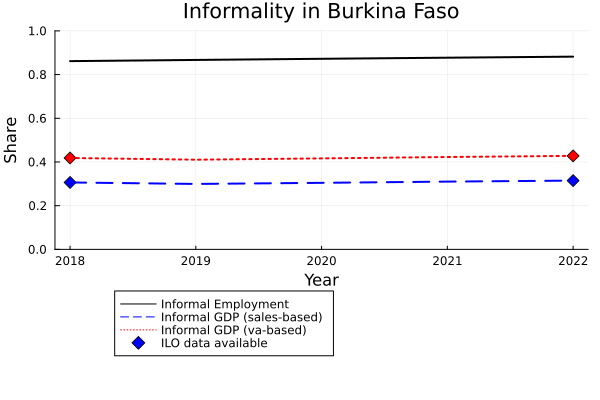
\includegraphics[width=\textwidth]{Burkina Faso.png}
        \end{subfigure}
        \hfill
        \begin{subfigure}[b]{0.49\textwidth}
            \centering
            \caption{}
            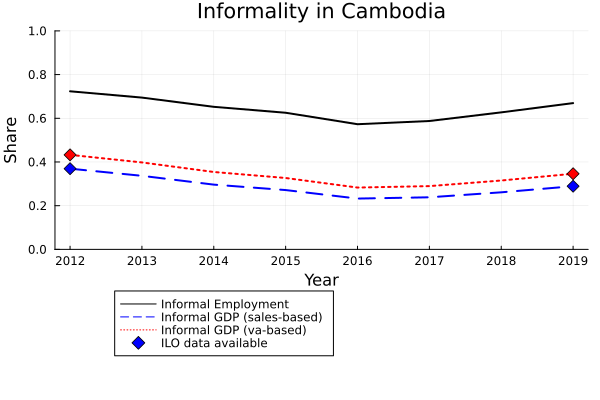
\includegraphics[width=\textwidth]{Cambodia.png}
        \end{subfigure}
        \caption*{\footnotesize The solid black line represents the share of employment operating outside the formal sector. The dashed blue line is the share of fiscal informality based on sales per worker calculations, while the dotted red line is based on value added per worker calculations. Diamonds indicate years in which informal employment data are available from ILO. When this information is not available, interpolated data are used. }    
    \end{figure}

    % \newpage 
    \begin{figure}[ht!]
        \centering
        \caption{Measures of Informality for Selected Countries}\label{info_ser_2}
        \begin{subfigure}[b]{0.49\textwidth}
            \centering
            \caption{}
            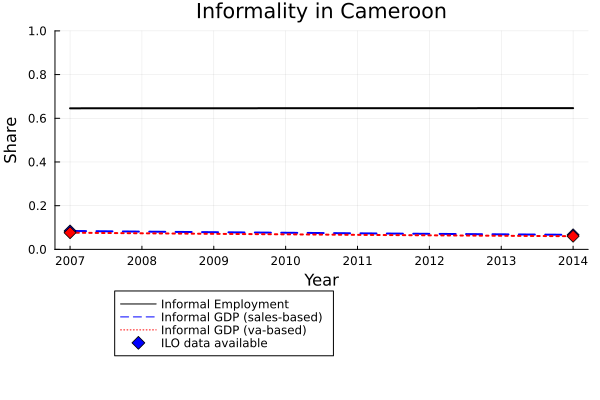
\includegraphics[width=\textwidth]{Cameroon.png}
        \end{subfigure}
        \hfill
        \begin{subfigure}[b]{0.49\textwidth}
            \centering
            \caption{}
            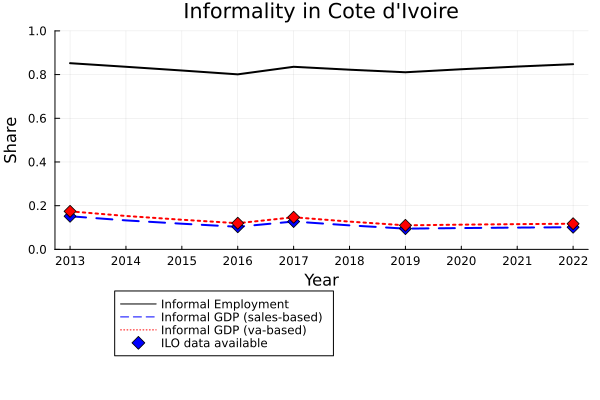
\includegraphics[width=\textwidth]{Cote d'Ivoire.png}
        \end{subfigure}
                \begin{subfigure}[b]{0.49\textwidth}
            \centering
            \caption{}
            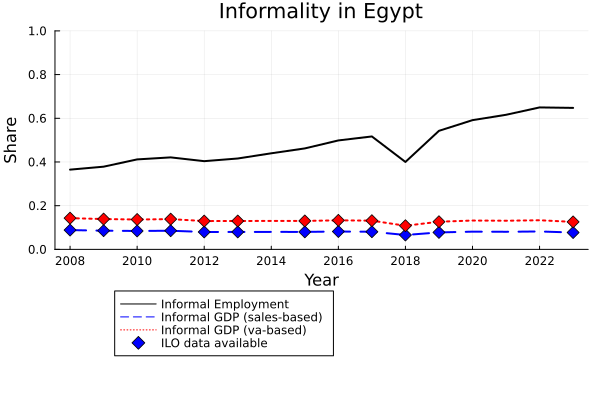
\includegraphics[width=\textwidth]{Egypt.png}
        \end{subfigure}
        \hfill
        \begin{subfigure}[b]{0.49\textwidth}
            \centering
            \caption{}
            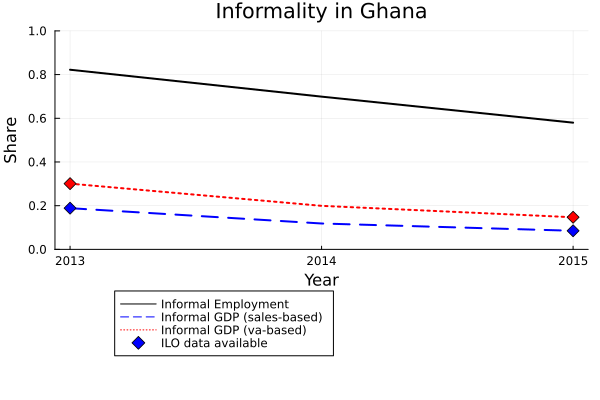
\includegraphics[width=\textwidth]{Ghana.png}
        \end{subfigure}
                \begin{subfigure}[b]{0.49\textwidth}
            \centering
            \caption{}
            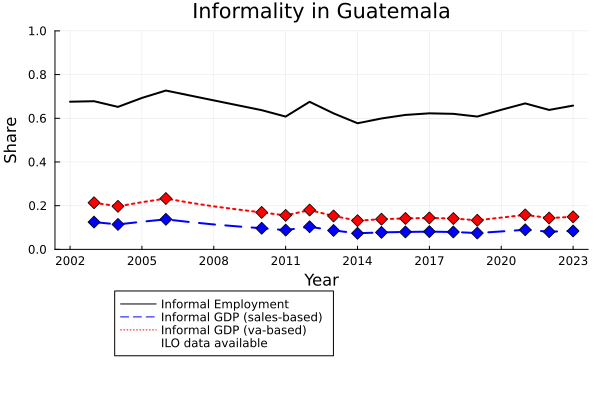
\includegraphics[width=\textwidth]{Guatemala.png}
        \end{subfigure}
        \hfill
        \begin{subfigure}[b]{0.49\textwidth}
            \centering
            \caption{}
            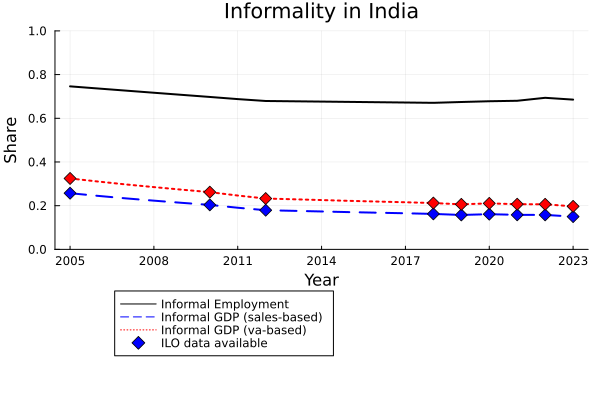
\includegraphics[width=\textwidth]{India.png}
        \end{subfigure}
        \caption*{\footnotesize The solid black line represents the share of employment operating outside the formal sector. The dashed blue line is the share of fiscal informality based on sales per worker calculations, while the dotted red line is based on value added per worker calculations. Diamonds indicate years in which informal employment data are available from ILO. When this information is not available, interpolated data are used. }    
    \end{figure}

    % \newpage 
    \begin{figure}[ht!]
        \centering
        \caption{Measures of Informality for Selected Countries}\label{info_ser_3}
        \begin{subfigure}[b]{0.49\textwidth}
            \centering
            \caption{}
            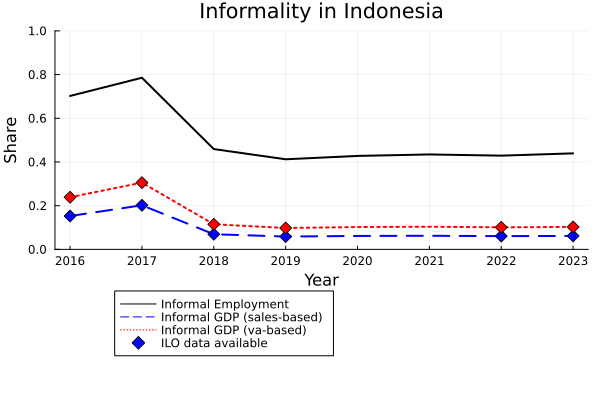
\includegraphics[width=\textwidth]{Indonesia.png}
        \end{subfigure}
        \hfill
        \begin{subfigure}[b]{0.49\textwidth}
            \centering
            \caption{}
            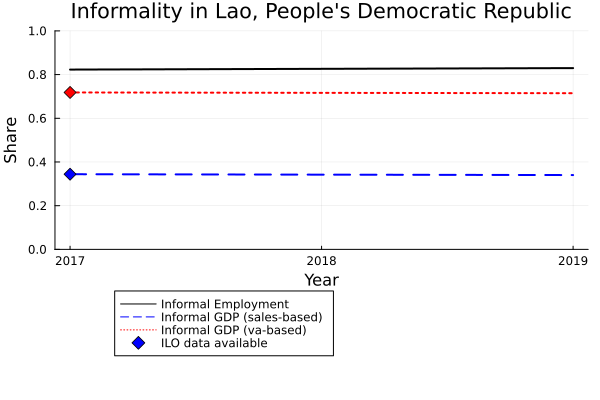
\includegraphics[width=\textwidth]{Lao, People's Democratic Republic.png}
        \end{subfigure}
                \begin{subfigure}[b]{0.49\textwidth}
            \centering
            \caption{}
            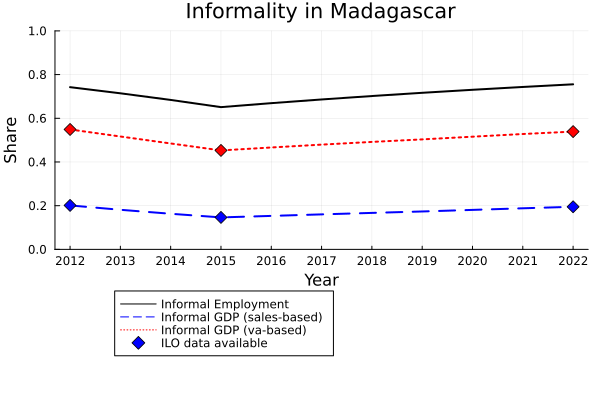
\includegraphics[width=\textwidth]{Madagascar.png}
        \end{subfigure}
        \hfill
        \begin{subfigure}[b]{0.49\textwidth}
            \centering
            \caption{}
            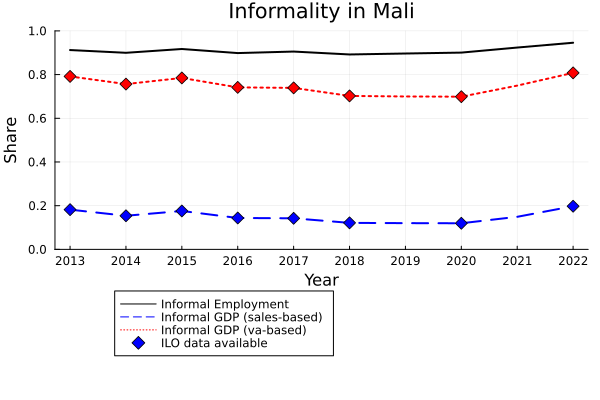
\includegraphics[width=\textwidth]{Mali.png}
        \end{subfigure}
                \begin{subfigure}[b]{0.49\textwidth}
            \centering
            \caption{}
            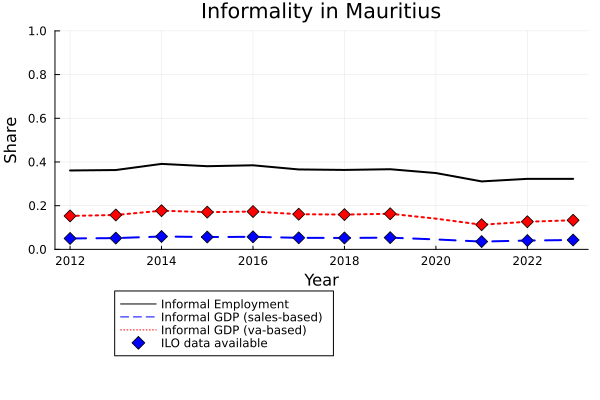
\includegraphics[width=\textwidth]{Mauritius.png}
        \end{subfigure}
        \hfill
        \begin{subfigure}[b]{0.49\textwidth}
            \centering
            \caption{}
            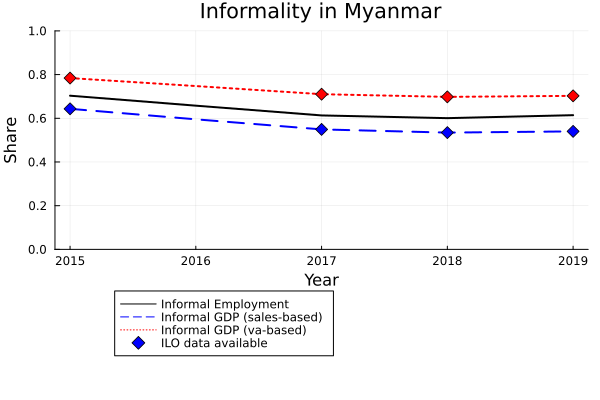
\includegraphics[width=\textwidth]{Myanmar.png}
        \end{subfigure}
        \caption*{\footnotesize The solid black line represents the share of employment operating outside the formal sector. The dashed blue line is the share of fiscal informality based on sales per worker calculations, while the dotted red line is based on value added per worker calculations. Diamonds indicate years in which informal employment data are available from ILO. When this information is not available, interpolated data are used. }    
    \end{figure}

    % \newpage 
    \begin{figure}[ht!]
        \centering
        \caption{Measures of Informality for Selected Countries}\label{info_ser_4}
        \begin{subfigure}[b]{0.49\textwidth}
            \centering
            \caption{}
            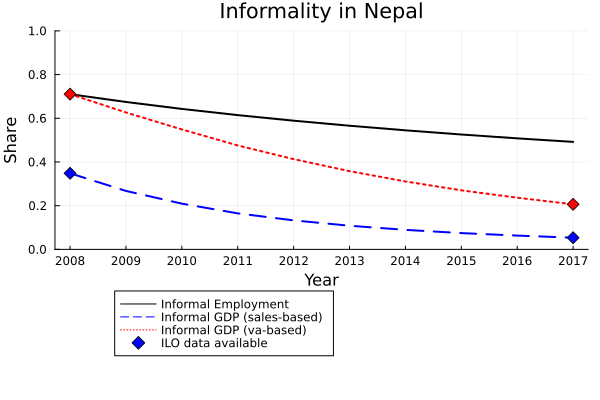
\includegraphics[width=\textwidth]{Nepal.png}
        \end{subfigure}
        \hfill
        \begin{subfigure}[b]{0.49\textwidth}
            \centering
            \caption{}
            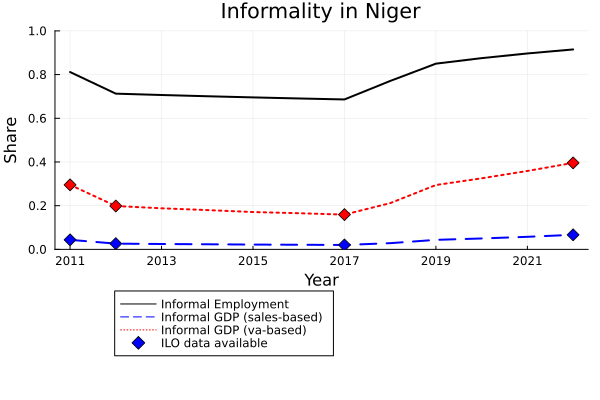
\includegraphics[width=\textwidth]{Niger.png}
        \end{subfigure}
                \begin{subfigure}[b]{0.49\textwidth}
            \centering
            \caption{}
            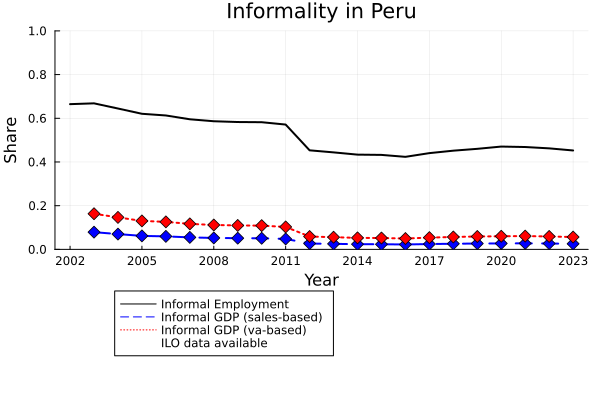
\includegraphics[width=\textwidth]{Peru.png}
        \end{subfigure}
        \hfill
        \begin{subfigure}[b]{0.49\textwidth}
            \centering
            \caption{}
            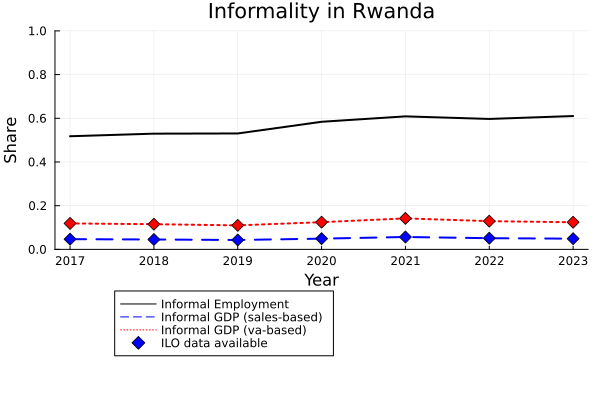
\includegraphics[width=\textwidth]{Rwanda.png}
        \end{subfigure}
                \begin{subfigure}[b]{0.49\textwidth}
            \centering
            \caption{}
            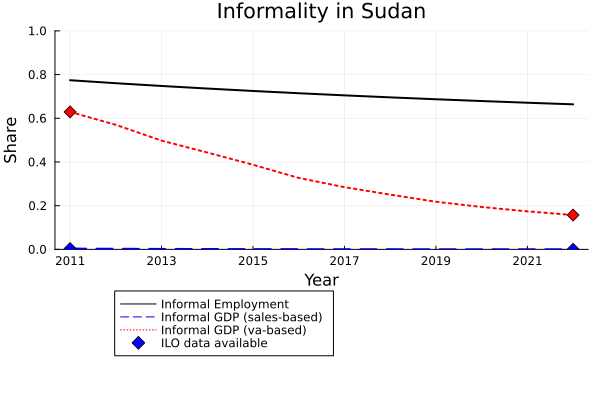
\includegraphics[width=\textwidth]{Sudan.png}
        \end{subfigure}
        \hfill
        \begin{subfigure}[b]{0.49\textwidth}
            \centering
            \caption{}
            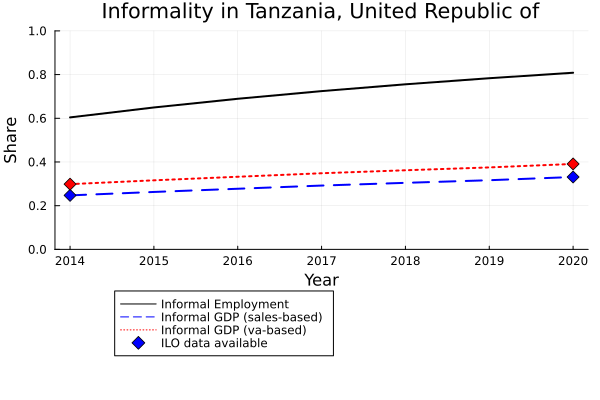
\includegraphics[width=\textwidth]{Tanzania, United Republic of.png}
        \end{subfigure}
        \caption*{\footnotesize The solid black line represents the share of employment operating outside the formal sector. The dashed blue line is the share of fiscal informality based on sales per worker calculations, while the dotted red line is based on value added per worker calculations. Diamonds indicate years in which informal employment data are available from ILO. When this information is not available, interpolated data are used. }    
    \end{figure}

        % \newpage 
    \begin{figure}[ht!]
        \centering
        \caption{Measures of Informality for Selected Countries}\label{}
        \begin{subfigure}[b]{0.49\textwidth}
            \centering
            \caption{}
            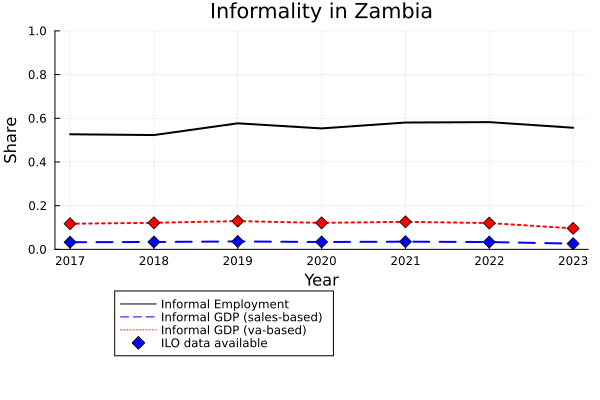
\includegraphics[width=\textwidth]{Zambia.png}
        \end{subfigure}
        \hfill
        \begin{subfigure}[b]{0.49\textwidth}
            \centering
            \caption{}
            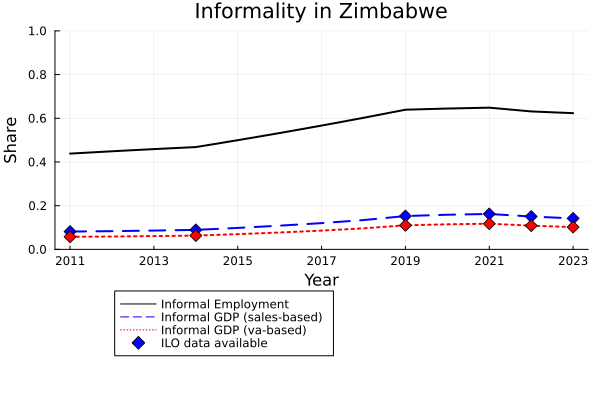
\includegraphics[width=\textwidth]{Zimbabwe.png}
        \end{subfigure}
        \caption*{\footnotesize The solid black line represents the share of employment operating outside the formal sector. The dashed blue line is the share of fiscal informality based on sales per worker calculations, while the dotted red line is based on value added per worker calculations. Diamonds indicate years in which informal employment data are available from ILO. When this information is not available, interpolated data are used. }
    \end{figure}

\noindent    
The following results stand out. First, in all countries except Myanmar, the share of informal employment is higher than the share of informal GDP (both sales- and VA-based), reflecting the higher average productivity of formal sector businesses. However, the magnitude of this discrepancy varies across countries. For instance, in Argentina and Peru, informal GDP accounts for less than 20\%, while informal employment hovers around or above 50\%. In contrast, several African and South/Southeast Asian countries exhibit narrower gaps between informal employment and informal GDP.
\\Second, sales-based informal GDP is generally lower than VA-based informal GDP. This pattern reflects a more intensive use of intermediate purchases by formal firms. Sales-based informal GDP tends to overstate the relative importance of the formal sector by not accounting for the relative higher share of intermediate purchases. Conversely, since data on intermediate purchases for informal businesses are rarely available (with electricity expenses used as a proxy when available), value added in the informal sector is likely to be overestimated. The two measures can be thought of as lower (sales-based) and upper (VA-based) bounds of the share of informal GDP.
\\Third, variations in informal GDP over time closely track variations in informal employment. While this feature partly occurs by construction, it represents an improvement over traditional measures of informal GDP, whose variations are generally driven by other macroeconomic statistics.
\\Finally, excluding short-term fluctuations, most countries display relatively steady informal GDP shares over the period considered, although a gradual decline is observed in a subset of countries.


    \subsection{Relationship Between Informal GDP and GDP per Capita}
    Figure \ref{corr_gdppc} displays the cross-country correlation between GDP per capita and sales-based (left panel) and VA-based (right panel) informal GDP. Each point represents a country-level average over the years for which the informality series is constructed, excluding data from 2020 on. Both panels show a negative correlation, consistent with previous studies documenting the prevalence of informality in low- and middle-income countries. 
    However, The charts also reveal a group of countries, mainly in Africa, with relatively low informal GDP despite very low income per capita. Three considerations should be taken into account. First, this pattern has been previously documented and is not in conflict with previous studies on informality measures. Various factors beyond income per capita, such as institutional differences, can affect the size of the informal sector. Second, the measure of informality used in this paper, legal informality, does not capture all dimensions of informality, such as tax evasion or informal employment within formal enterprises. Third, for countries surveyed before 2016, firm-level data may not be representative of the business population, which could lead to flawed informal GDP measures.  

    \begin{figure}[ht!]
        \centering
        \caption{Relationship Between Informal GDP and GDP per Capita}\label{corr_gdppc}
        \begin{subfigure}[b]{0.49\textwidth}
            \centering
            \caption{}
            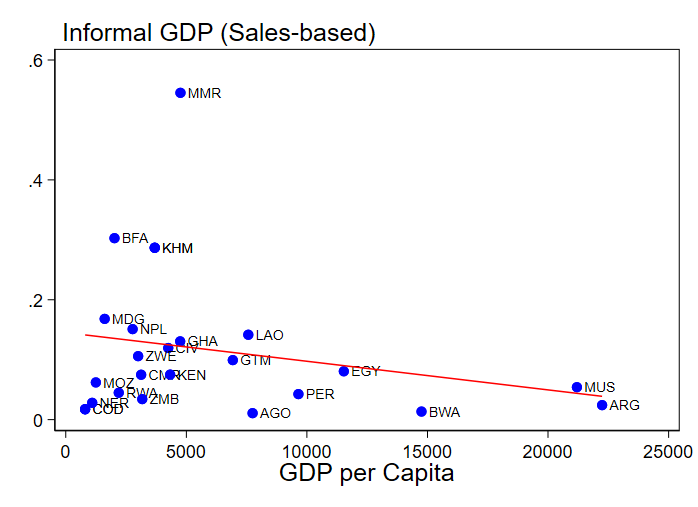
\includegraphics[width=\textwidth]{corr_gdppc_1.png}
        \end{subfigure}
        \hfill
        \begin{subfigure}[b]{0.49\textwidth}
            \centering
            \caption{}
            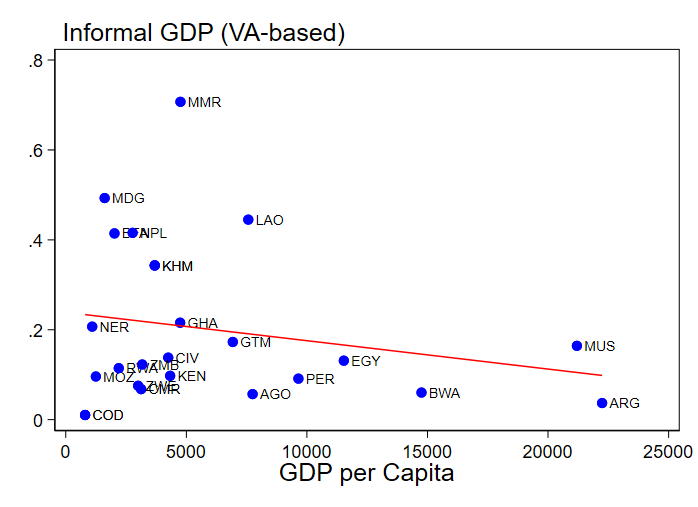
\includegraphics[width=\textwidth]{corr_gdppc_2.png}
        \end{subfigure}
        \caption*{\footnotesize Source: Own calculation for informal GDP, PWT for GDP per capita. Each point represents an average over the years shown in Figures \ref{info_ser_1} to \ref{info_ser_4}, with the exclusion of the years from 2020 on. }
    \end{figure}

    \subsection{Relationship Between Informal GDP Change and GDP Growth Rates}
    Several studies have documented the countercyclical nature of informality, Particularly its tendency to increase during recessions.\footnote{For example, \textcolor{blue}{\textcite{leyvaurrutia2020}} and \textcolor{blue}{\textcite{pappadarogoff2025}}.} These studies generally employ detailed country-specific information collected at the household or firm level, or both. Ideally, time series of informality should preserve this feature. Figure \ref{corr_gdpgr} illustrates the correlation between GDP growth and changes in sales-based (left panel) and VA-based (right panel) informal GDP. Each point represents a combination of GDP growth and change in informal GDP for a given country-year. Both panels display a negative correlation, suggesting that the measures constructed capture the countercyclical behavior of informality.

    \begin{figure}[ht!]
        \centering
        \caption{Relationship Between Informal GDP Change and GDP Growth Rates}\label{corr_gdpgr}
        \begin{subfigure}[b]{0.49\textwidth}
            \centering
            \caption{}
            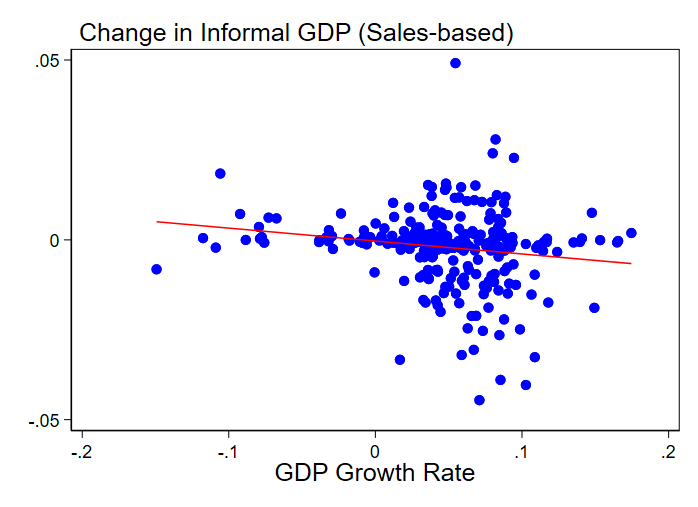
\includegraphics[width=\textwidth]{corr_gdpgr_1.png}
        \end{subfigure}
        \hfill
        \begin{subfigure}[b]{0.49\textwidth}
            \centering
            \caption{}
            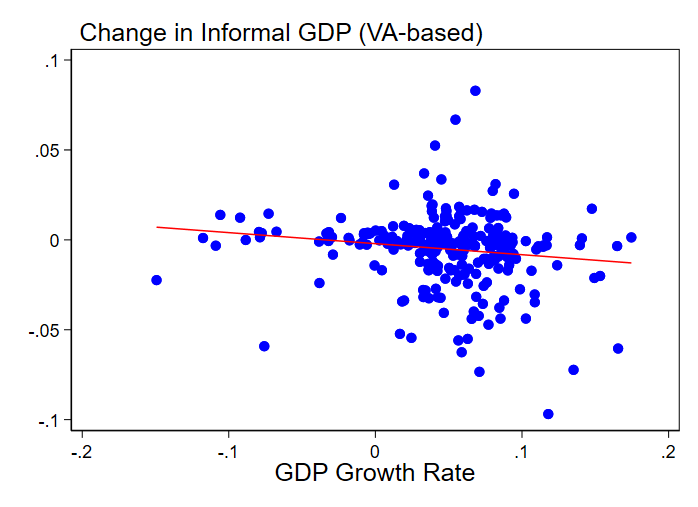
\includegraphics[width=\textwidth]{corr_gdpgr_2.png}
        \end{subfigure}
        \caption*{\footnotesize Source: Own calculation for informal GDP, PWT and World Bank for GDP growth. For visualization purposes, I exclude from the graph a couple of outliers (they are not excluded from the empirical analysis). }
    \end{figure}

    \noindent
    To test this relationship more formally, I run the following regressions:

    $$\Delta S_{O,t} = \alpha + \beta \Delta GDP_{t} + \varepsilon_{t} $$

    \noindent
    Where $\Delta S_{O,t}$ is the annual change in either sales-based or VA-based informal GDP, $\Delta GDP_{t}$ is the annual GDP growth, and $\varepsilon$ is an error term. 
    \\Table \ref{tab_gdpgr} displays the estimates of the coefficient $\beta$, the sensitivity of informal GDP changes to GDP growth. The coefficients are negative, as predicted, and statistically significant at the 10\% level.

    \begin{table}[ht!]
        \centering
        \caption{Relationship Between Informal GDP Change and GDP Growth Rates}\label{tab_gdpgr}
        {\def\sym#1{\ifmmode^{#1}\else\(^{#1}\)\fi}
        \begin{tabular}{l*{2}{c}}
            \hline\hline
            &Informal GDP Change       &Informal GDP Change               \\
            &(sales-based)       &(VA-based)                \\
            \hline
            GDP Growth      &     -0.032\sym{*} &      -0.057\sym{*} \\
                    &     (0.019)         &     (0.031)         \\
            % GDP Growth&                     &           \\
            %         &                     &                       \\
            \hline
            Observations        &      144         &      144         \\
            \hline\hline
            \footnotesize Standard errors in parentheses\\
            \footnotesize \sym{*} \(p<.10\), \sym{**} \(p<.05\), \sym{***} \(p<.01\)\\
            \end{tabular}
        }            
    \end{table}

        \subsection{Comparison With Existing Measures of Informal GDP}
        Table \ref{tab_comp} compares country averages across different estimates of informal GDP. Columns (1) and (2) report the sales-based and VA-based informal GDP derived in this paper, while columns (3) and (4) show the DGE and MIMIC estimates from \textcolor{blue}{\textcite{elginetal2021}}. For each country, averages are computed only for the years in which all four series are available.
        \\The measures estimated in this paper tend to be lower than those reported previously. As shown in the bottom row of table \ref{tab_comp}, the cross-country averages for sales-based and VA-based informal GDP are about 13\% and 23\%, compared to 34\% and 39\% for the DGE and MIMIC estimates. Several factors may explain this discrepancy. First, this paper focuses on a narrower dimension of informality, legal informality, which captures only the production of unregistered businesses, excluding unreported production by otherwise formal enterprises. Second, the analysis is restricted to the non-agricultural sector, which typically exhibits lower levels of informality than the agricultural sector. Third, the exclusion of formal firms with less than five employees in the WBES may lead to an overestimation of the formal sector average productivity, thereby underestimating the share of informal GDP. Conversely, the WBES may also fail to detect very large and highly productive formal firms. As a result, it is not ex-ante clear which effect prevails.

       \begin{table}[ht]
        \footnotesize
        \centering
                \caption{Country Averages by Measures of Informal GDP}\label{tab_comp}
        \begin{tabular}{l l | p{2cm} p{2cm} | p{2cm} p{2cm}}
        \hline
        \hline
        &  & (1) & (2) & (3) & (4) \\
        \textbf{Country} & \textbf{Years} & \textbf{Sales-Based} & \textbf{VA-Based} & \textbf{DGE} & \textbf{MIMIC} \\
        \hline
        \hline
        Angola & 2004-2018 & 1.1\% & 5.6\% & 40.8\% & 44.4\% \\
        Argentina & 2004-2018 & 2.4\% & 3.7\% & 22.3\% & 24.4\% \\
        Bangladesh & 2010-2018 & 22.6\% & 46.6\% & 30.2\% & 35.1\% \\
        Botswana & 2006-2018 & 1.3\% & 6.0\% & 29.7\% & 30.9\% \\
        Burkina Faso & 2018-2018 & 30.6\% & 41.8\% & 31.6\% & 38.7\% \\
        Cambodia & 2012-2018 & 28.7\% & 34.3\% & 40.0\% & 46.0\% \\
        Cameroon & 2007-2014 & 7.5\% & 6.8\% & 30.9\% & 32.2\% \\
        % Congo, The Democratic Republic of & 2005-2018 & 1.7\% & 1.1\% & 45.2\% & 47.0\% \\
        Cote d'Ivoire & 2012-2018 & 12.4\% & 14.3\% & 44.9\% & 41.9\% \\
        Egypt & 2008-2018 & 8.1\% & 13.2\% & 31.2\% & 34.2\% \\
        Ghana & 2013-2015 & 13.1\% & 21.6\% & 37.9\% & 39.2\% \\
        Guatemala & 2002-2018 & 10.1\% & 17.5\% & 47.6\% & 51.9\% \\
        India & 2005-2018 & 19.7\% & 25.4\% & 19.3\% & 21.1\% \\
        Indonesia & 2016-2018 & 14.1\% & 22.0\% & 15.7\% & 18.4\% \\
        Lao, People's Democratic Republic & 2017-2018 & 14.6\% & 45.4\% & 21.8\% & 28.2\% \\
        Madagascar & 2012-2018 & 16.7\% & 49.2\% & 36.9\% & 43.4\% \\
        Mauritius & 2012-2018 & 5.4\% & 16.5\% & 20.5\% & 21.6\% \\
        Mozambique & 2015-2015 & 6.2\% & 9.6\% & 28.2\% & 39.0\% \\
        Myanmar & 2015-2018 & 54.6\% & 70.8\% & 26.6\% & 49.1\% \\
        Nepal & 2008-2017 & 15.1\% & 41.6\% & 34.6\% & 36.4\% \\
        Niger & 2011-2018 & 2.6\% & 19.6\% & 37.0\% & 40.2\% \\
        Peru & 2002-2018 & 4.4\% & 9.3\% & 50.9\% & 57.2\% \\
        Rwanda & 2017-2018 & 4.6\% & 11.7\% & 29.2\% & 35.4\% \\
        Sudan & 2011-2018 & 0.2\% & 42.4\% & 20.8\% & - \\
        Tanzania, United Republic of & 2014-2018 & 27.7\% & 33.1\% & 45.9\% & 54.2\% \\
        Zambia & 2017-2018 & 3.3\% & 12.0\% & 40.6\% & 47.2\% \\
        Zimbabwe & 2011-2018 & 10.0\% & 7.1\% & 64.0\% & 60.7\% \\
        \hline
        Cross-Country Average &  & 12.6\% & 23.3\% & 34.2\% & 39.1\% \\
        \hline
        \hline
        \end{tabular}
        \caption*{\footnotesize Source: Own calculation for columns (1) and (2), \textcolor{blue}{\textcite{elginetal2021}} for columns (3) and (4).}
    \end{table}

    \section{Conclusion}\label{sec_concl}
    This paper provides a method to estimate the share of informal GDP using a simple framework and data from various surveys and sources. The estimated informality series exhibit three key features: (i) a negative correlation with GDP per capita, (ii) mild anticyclical behavior, (iii) lower levels than those reported in previous cross-country studies. While the current approach allows estimation for only a subset of countries and years, it offers a foundation for future research. Subsequent work could expand the time span, the number of countries, or both. Although the number of countries is constrained by the availability of informal WBES, the time dimension could be extended by incorporating country-specific labor force surveys in place of ILO data.


% \section{Model}
% I rely on the deterministic dynamic general equilibrium model developed by {\textcite{elginoztunali2012}}. In the model, an infinitely-lived representative household is endowed with an initial level of capital $K_0$ and a labor endowment $H_t>0$. There exist two different production technologies transforming production factors into a homogeneous final good: the \textit{formal} sector technology, which employs capital and labor, and the \textit{outside formal} sector technology, which only employs labor.
% The representative household chooses consumption, investment, and the allocation of labor between the formal and outside formal sector to maximize their lifetime utility.
% \\Formally, the household solves the following dynamic program:

% % Requires: \usepackage{amsmath}
% \begin{align}
%     \max_{\{C_t, K_{t+1}, N_{Ot}, N_{Ft}\}_{t=0}^{\infty}} \ \ \sum_{t=0}^{\infty} \beta^t U(C_t)& \label{dyn_pro}\\
%     \text{s.t.} \ \ \ \  C_t + K_{t+1} &= (1-\delta)K_t + (1-\tau_t)\theta_{Ft} K_t^\alpha N_{Ft}^{\gamma_F} + \theta_{Ot} N_{Ot}^{\gamma_O} \\
%      \quad N_{Ot} + N_{Ft} &= H_t.
% \end{align}
% \noindent
% Where $C_t$, $K_t$, $N_{Ft}$, $N_{Ot}$ denote consumption, capital, employment in the formal sector, and employment outside the formal sector, 
% $\theta_{Ft}$ and $\theta_{Ot}$ denote aggregate productivity in the formal and outside the formal sector, $\alpha$, $\gamma_F$ and $\gamma_O$ denote production factors' shares, $\tau_t$ is the formal output tax rate, and $\beta$ and $\delta$ represent the discount factor and the depreciation rate, respectively. $U(\cdot$) is an increasing and concave function satisfying the usual properties.
% Besides the differences in production technologies, the assumption in the model is that producers outside the formal sector can hide their output costlessly, so that the output tax is only applied to formal producers. The revenues collected are used to finance government expenditures $G_t$ that do not enter in the household's utility function.

% \vspace{3mm}
% \noindent
% \textbf{Equilibrium.} Given $K_0$ and a sequence of tax rates $\tau_t$, a competitive equilibrium is defined as a sequence of consumption, capital, employment in the formal and outside formal sector, and public expenditures $\{C_t, K_{t+1}, N_{Ft}, N_{Ot}, G_t\}_{t=0}^\infty$ such that (i) the household solves the dynamic program \ref{dyn_pro} and (ii) the government balances its budget in each period $G_t=\tau_t\theta_{Ft} K_t^\alpha N_{Ft}^{\gamma_F}$.

% \vspace{3mm}
% \noindent
% \textbf{Equilibrium Characterization.} The equilibrium is characterized by the following three equations\footnote{I assume that $U(c)=log(c).$}
% \begin{align}
%         \frac{C_t}{C_{t-1}}&=\beta[(1-\delta)+(1-\tau_t)\alpha\theta_{Ft}K_t^{\alpha-1}N_{Ft}^{\gamma_F}] \label{Euler}\\
%         \gamma_F(1-\tau_t)\theta_{Ft}K_t^\alpha N_{Ft}^{\gamma_F-1}&=\gamma_O\theta_{Ot}N_{Ot}^{\gamma_O-1}\label{lab_eq}\\
%         G_t&=\tau_t\theta_{Ft} K_t^\alpha N_{Ft}^{\gamma_F}\label{govt_eq}
% \end{align}
% Equation (\ref{Euler}) is the Euler equation. Equation (\ref{lab_eq}) equates the marginal product of labor in the formal sector to the marginal product of labor outside the formal sector. Finally, equation (\ref{govt_eq}) reflects the government budget balance.

% \section{Calibration}
% In addition to equations (\ref{Euler}) to (\ref{govt_eq}), I employ three equations who allow me to pin down the key model's parameters through the use of micro data:
% \begin{align}
%     \frac{\theta_{Ft}}{\theta_{Ot}}&=\mu_t\label{prod_ratio}\\
%     \frac{\gamma_{Ft}}{\gamma_{Ot}}&=\nu_t\label{gamma_ratio}\\
%     Y_t&=\theta_{Ft} K_t^\alpha N_{Ft}^{\gamma_F} + \theta_{Ot} N_{Ot}^{\gamma_O}\label{output_eq}    
% \end{align}
% Equation (\ref{prod_ratio}) pins down the ratio between the TFP terms in the formal and outside the formal sector, while Equation (\ref{gamma_ratio}) pins down the ratio between the labor shares in the two sectors. Both ratios $\mu_t$ and $\nu_t$ are estimated using firm-level data from the World Bank Enterprise Survey.
% Equation (\ref{output_eq}) defines output. 
% \\The macroeconomic variables are taken from three main sources. I take the sequence for consumption, capital, public expenditures, and output from the \textit{Penn World Table (PWT)} or from the \textit{World Bank}\footnote{The most recent data from PWT are for 2019, therefore I use the World Bank data for for any years after 2019, making sure that the series are consistent across the two different sources.}. I also estimate country-specific depreciation rates $\delta$ from PWT by taking an average over the relevant period. The figures for employment in the formal sector and outside the formal sector are taken from the \textit{International Labour Organization (ILO)}. The ILO provides data on employment only for some of the years within a period, therefore, I perform linear interpolation whenever necessary. Finally, the capital share $\alpha$ is set equal to $0.3$.
% \\Six variables remain to be calibrated within the model: the discount factor $\beta$, the labor shares $\gamma_F$ and $\gamma_O$, the TFP terms $\theta_{Ft}$ and $\theta_{Ot}$, and the tax rate $\tau_t$. Equations (\ref{Euler}) to (\ref{govt_eq}) allow me to calibrate these variables.

\newpage
\printbibliography

\newpage

\section*{Appendix: WBES Data}\label{app_wbes}
\textbf{Description of data.} Firm-level data from the WBES are available at
\href{https://www.enterprisesurveys.org/en/data}{https://www.enterp-}
\href{https://www.enterprisesurveys.org/en/data}{risesurveys.org/en/data}. The data portal provides a comprehensive database covering formal business with at least five employees across countries and survey years. For most observations, the following key variables are available: annual sales, annual cost of intermediate purchases, value of capital, number of employees, industry classification (manufacturing or services), and country-specific sample weights. I exclude from the sample any observations with missing values for these variables. These data allow me to compute the (weighted) average sales and value added per worker —used on the right hand side of equation (\ref{vapw_form})— and estimate the production factor shares of equation (\ref{eq_prod_form}). 
\\The data portal also includes a combined database of the most recent informal surveys, which contain the same variables as the standard WBES, except for the value of capital and expenditures on intermediate purchases. To expand country coverage, I harmonize and merge data from informal surveys conducted prior to 2016. Unfortunately, sample weights are not available for these earlier surveys. In such cases, I assign equal weights to all observations within a country.
Given the absence of firm-level data on intermediate purchases in the informal sector, I use annual electricity expenditures as a proxy and subtract them from annual sales to compute value added. In Section \ref{sec_results}, I discuss the implications of this choice. 
\\
\\\textbf{Data cleaning.} Monetary values for sales and capital are expressed in local currencies. To ensure consistency across countries and with other macroeconomic variables from the PWT, I convert all monetary variables to constant 2017 USD. This conversion involves two steps: first, I use average annual exchange rates from the World Bank to convert current local currency values into current USD; second, I apply deflators from the Federal Reserve Economic Data (FRED) to express these values in constant 2017 USD.
\\Additionally, I exclude a small number of observations where a single firm's value added exceeds the sum of the value added of all other firms in the same country. While these large firms may exist, their inclusion would distort the estimation of average sales and value added per worker. Of the 26 countries considered, only seven observations are excluded, three from the formal sector and four from the informal sector.
\\Finally, I replace estimated production factor shares $\hat{\alpha}$, $\hat{\gamma_F}$, and $\hat{\gamma_O}$ with cross-country averages whenever their estimated values are negative. This adjustment is applied in three cases: twice for formal sector shares (Angola and Lao PDR), and once for informal sector labor share (Cambodia).
\\
\\
\textbf{Representativeness of the data.} How do informal sector surveys ensure representativeness of the population of informal businesses? Typical informal businesses do not appear in official registrar records or tax rolls. To address this, \textcolor{blue}{\textcite{agaetal2022}} propose a methodology based on Adaptive Cluster Sampling (ACS), which generates a representative sample of informal businesses using a geographic sampling approach. This method consists of the following two stages: in the first stage, ACS provides a probabilistic sample of surveyed units which are fully enumerated to list all informal businesses. In the second stage, businesses are randomly selected from the list for an interview.





\end{document}
